%%--------------------------------------------------
%\subsection{Traffic Simulation}
%\label{ss:Traffic Simulation}
%% - - - - - - - - - - - - - - - - - - - - - - - - -
%(Hattori, Ito?)

Car traffic is one of popular targets of social simulations, and it is applied to various objectives, for example, traffic control, city design, economic activities, and 
environmental issues. In this CASSIA project, some traffic simulations and their analyses have been achieved not only in applications and also in basic modelings, applying and assuming 
present and future supercomputers. 

\paragraph{Simulation cost and benchmark}

Traffic simulations are comprised of three parts: road map with traffic rules and regulations, 
origin and destination(OD) sets of cars with travel routes, and movements of cars on the map 
along their routes. 
There are two method to parallelize traffic simulations. One is to parallelize geometrically, and the other car- or trip-wisely. 
Geometrical parallelization is advantageous on modern supercomputers, because necessary data transfer is states of cars which move out from an area on one node and go to an area on other node, 
and only nearest-neighbor communications appear. 

Parallelization of trip routings is more complicated but most trips are short range and are executed on one node using local map. 
Time comsuming long trips are few, and their routing cost can be made negligible. 

Simulation of car movements can be made very simple and also very complicated. In case of normal traffic without hazardous conditions like accidents or disasters, 
it is sufficient to execute few arithmetic operations per car using distance to a car in front and legal speed limit, which determe appropriate velocity that the car does not crash to 
a car in front and does not break the legal limit. 
To the contrary, heavy operations are necessary to simulate high-resolution movements of car to study, for example, risk of traffic accidents and weather effects. 
Hydrodynamic and/or machine engineering simulations solving PDE with high reliability in space and time will be executed. In this extreme, simulations of just one car may require 
Exa-scale computers. 

Parallelization feature of car traffic simulations with the most parallelization demanding case, that is, simulations using the simplest car movement was measures in this CASSIA project. 
Each car continues to move along road, and turn randomly at each crossing. This means that no routing is done. This simulation model will require the lightest processing 
in each computer node, and the most frequent  inter-node communication. 
Results of strong scaling of parallelized performance using the K computer up to its quarter configuration(20,736 nodes) for the traffic simulation on entire road of Japan are shown
 in Fig.~\ref{itoallJapan}. 
Simulations were up to 100 second and time step was 0.01 second. So totally 10,000 steps were done for about 11.7 million cars on totally 1.28 million kilometer-long  roads 
using the ``Open Street Map''. Using the quarter nodes, simulations of 10,000 steps were executed in 11.5 second apart from the initial preparation(66.1 second), 
and efficient parallelization is confirmed. 
For another simulation of 100 million car on all-over the world with 30.9 million kilometer took 116 second using quarter nodes of the K computer. 

This result implies that realtime or faster car-traffic simulation will be executed on the K and the future supercomputers. 

\begin{table}
 \centering
  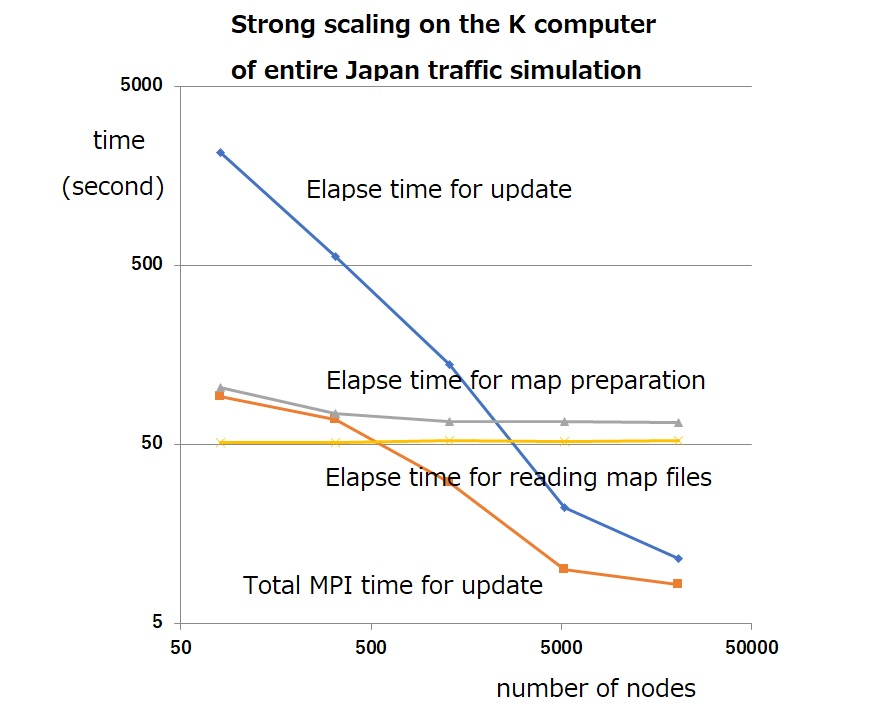
\includegraphics[width=.5\linewidth]{Figs.ito/allJapan.jpg}
  \caption{Results of strong scaling using the K computer for entire Japan traffic simulation with the simplest movements without routings are plotted.   }
  \label{itoallJapan}
\end{table}

\paragraph{Traffic factors}

In traffic simulation models, numbers of input parameters and output results are enormous. Each car has several input parameters, for example, its origin, destination, 
starting time, driving preference and also several output parameters, for example, travel duration and gas consumption. 
Each traffic signal has its control parameters. Each road segment has its speed limit and car flux. 
Such parameter-number explosion is quite common in various social models. 
In Kobe city, as an example, there are more than 30,000 road segments and about 100,000 trips(OD pairs) daily. So the number of input parameters 
and output results are order of $10^5$ at least. 
Without knowing behavior of simulation model, we cannot apply the model to describe, predict and design the real phenomena. 
But it is impossible to tame a model with $10^5$ input and output. 
So the first step is to eliminate unimportant parameters and to extract relevant parameters. 
A standard method for this purpose is the multivariate statistical analysis. 

In this CASSIA project, a car-traffic model and simulator of Kobe city was developed[Ito1]. Using this simulator, Monte Carlo simulations for various OD sets satisfying a constraint 
that daily trips be 100,000 and 70\% of the trips are coming from peripheral cities and just passing through Kobe city. A factor analysis was applied to the output flux of road segments[Ito2].  
Numbers of estimated factors are plotted in Fig.~\ref{itoFactor}. It is observed in this Fig.~\ref{itoFactor} that thousands of samples finally clarifies hundreds of factors. 
Hundreds are still large, but anyway we succeeded to extract relevant factors. 

This is still a model analysis, but this result will suggest that we will need to measure traffic thousands times to extract the relevant factors from real traffic phenomena, 
but real traffic will never repeat the same traffic thousands times. So we can use plausible computer simulation models to get better description of the real social phenomena. 

\begin{table}
 \centering
  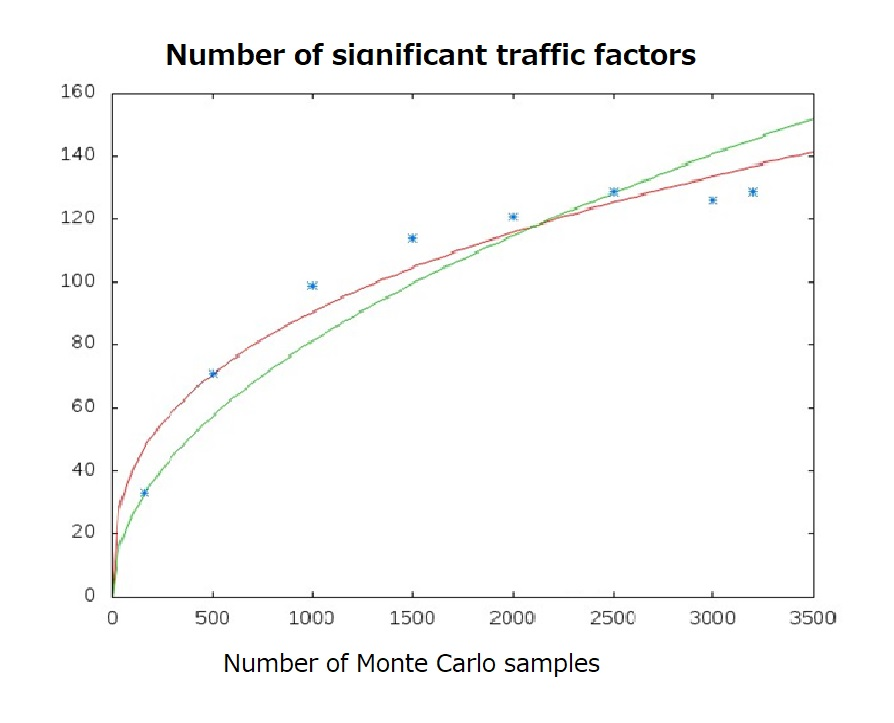
\includegraphics[width=.5\linewidth]{Figs.ito/Factors.jpg}
  \caption{Number of factors estimated using a factor analysis are plotted. Green curve shows square root of number of Monte Carlo samples, which is expected in the case of uniform 
distribution of eigenvalues of correlation matrix, but this plot is interpolated by slower red curve. }
  \label{itoFactor}
\end{table}

\newpage

\noindent {\bf References}

\noindent [Ito1]Yuta Asano, Nobuyasu Ito, Hajime Inaoka, Tetsuo Imai and Takeshi Uchinane, Proceedings of the International Conference on Social Modeling and Simulation, plus Econophysics Colloquium 2014(Springer Proceedings in Complexity, ISBN 978-3-319-20590-8), p. 255-264, 
{\it Traffic Simulation of Kobe-City}. 

\noindent [Ito2]Takeshi Uchitane and Nobuyasu Ito, "Applying Factor Analysis to Describe Urban Scale Vehicfle Traffic Simulation Results," (in Japanese) 
Journal of the Society of Instrument and Control Engineers vol.52 (2016) No.10 p.545-554. 

%[Ito1] Hideyuki Mizuta, Takashi Imamichi, �gLarge-scale social simulation framework "X10-based Agent Simulation on Distributed Infrastructure (XASDI)�h and applications�h, AROB 23nd 2018 , B-Con PLAZA, Beppu. JAPAN ,Jan. 19, 2018.
